\subsection{Exploring the game world}
The game starts in one of the various "landscapes" such as a desert, a forest, etc. each characterized by different terrain generation parameters and colors.

To make exploring the game world easier, the player can get into a car that moves considerably faster than the player.
\autoref{fig:car-in-hyperbolic} shows the car driving in hyperbolic space.
\begin{figure}[!htb]
    \centering
    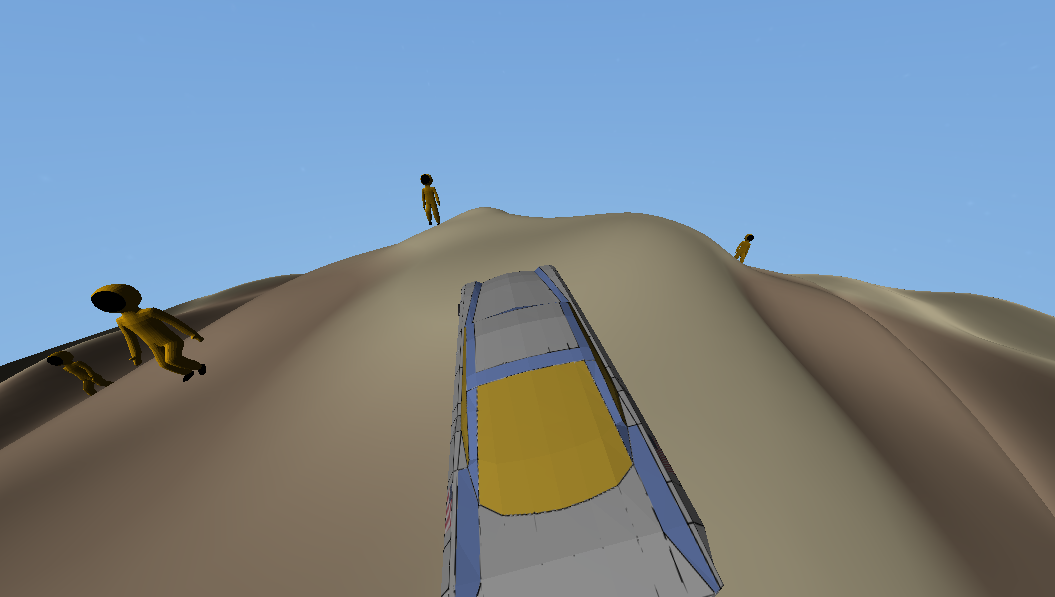
\includegraphics[width=0.8\textwidth]{chapters/results/sections/gameplay/resources/car-in-hyperbolic.png}
    \caption{Riding a car in hyperbolic space}
    \label{fig:car-in-hyperbolic}
\end{figure}
Even though the car is much faster than the player it can roll over when traversing a particularly bumpy terrain.
For this reason, we included an option to flip the car back on its wheels when that happens.